\documentclass{article}
\usepackage{graphicx}
\usepackage{amsmath}
\usepackage{algorithm}
\usepackage[noend]{algpseudocode}
\usepackage{amsfonts}


\title{Streamdice: An encryption algorithm based on catalogued shuffled keyboards}
\author{Andrew R. Garcia\\garcia.gtr@gmail.com}
\date{}

\begin{document}

\maketitle

\begin{abstract}
The algorithm presented in this paper is a stream cipher that provides encryption by considering the specific 
identity of characters and their relative location in the message. \texttt{STREAMDICE} uses shuffled keyboards,
generated by a pseudo-random number generator (PRNG), with each keyboard shifted for every encrypted character. 
These shuffled keyboards are stored in memory using seeds, which are dependent on the provided encryption keys. 
The periodicity of the algorithm is obscured by the pseudo-random factor, and the encryption operations make it resistant to brute force attacks. 
The algorithm shuffles the keyboard with each new character encryption, allowing for repeated permutations. 
The specific seeds used for keyboard generation are computed from the user-provided encryption keys. 
The decryption process reverses the encryption protocol using the same keys. This approach optimizes auxiliary space complexity.

\end{abstract}

\section{Introduction}
Good encryption can be used to protect data and private information. 
When properly encrypted, even if data is accessed in an unauthorized manner or unwillingly disclosed, 
the non-consented reader will be unable to read it without the correct encryption keys. The algorithm presented here, \texttt{STREAMDICE}, 
is a stream cipher which encrypts characters (i.e. letters, numbers and some allowed signs) by both their specific identity as well as their 
relative location in the message thread. For streamdice, the stream units are shuffled keyboards generated by a pseudo-random number generator
(PRNG), each of which are shifted once for every single encrypted character. The shuffled keyboards are limited and kept in memory
with seeds, which are in turn dependent on the provided keys for encryption. The pseudo-random factor obfuscates the periodicity 
of the algorithm, and the encryption operations make it challenging to exploit by brute force.

\section{Method}

In short, the algorithm starts by initializing an unwarped map of QWERTY characters. 
This keyboard map is then warped through character shuffling to produce a new arrangement. 
Each shuffling operation is linked to a number associated with the PRNG seed. 
For any given string or message, the algorithm encrypts each character using this method, that is,
applying one keyboard warp per character. In this sense, \texttt{STREAMDICE} combines elements of both a stream cipher and a block cipher. 
The sections below give a more detailed explanation of these steps.



\subsection{Unwarped Map Creation}
The unwarped map represents the original arrangement of characters on the keyboard. Let \( \Xi \) be the
character set used for encryption. The character set is in a sense the QWERTY keyboard (Figure \ref{fig:keyboard}), 
including uppercase and lowercase letters, numbers, and special characters. 
The bidirectional map is tied to map unwarping \( \mathcal{U} \), that associates each character \( \Xi_i \) in the character set \( \Xi \) 
with its corresponding index \( i \), such that:

\begin{align}
    \mathcal{U} = \{ (\Xi_i, i) \, | \, \forall i \, (\Xi_i \in \Xi) \}
\end{align}

and its inverse:

\begin{align}
    \mathcal{U}^{-1} = \{ (i, \Xi_i) \, | \, \forall i \, (i \in \mathbb{N}) \}
\end{align}


\begin{figure}[h]
  \centering
  \includegraphics[width=0.7\linewidth]{img/qwerty.png}
  \caption{Standard QWERTY keyboard}
  \label{fig:keyboard}
\end{figure}


\subsection{Map Warping}
The map warping operation \( \mathcal{W} \) is initialized with a  \( \text{PRNG}(\mu_i) \) seeding, 
where \( \mu_i \) is a seed generated by the encryption key provided by the user, and then re-shuffling all keys. 
This operation adds a layer of randomness to the encryption process. It should be known that every map warping operation
produces a unique keyboard set (Figure \ref{fig:hash}).


\begin{figure}[h]
  \centering
  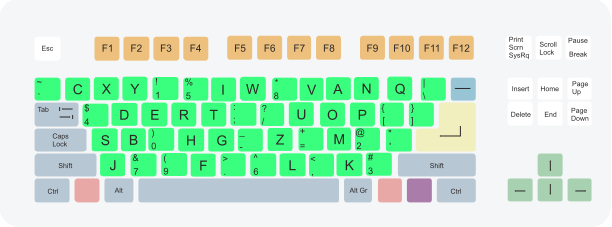
\includegraphics[width=0.7\linewidth]{img/qwerty_shuffled.png}
  \caption{Randomly-shuffled keyboard with $\mu_i$ seed \#5443}
  \label{fig:hash}
\end{figure}



\subsection{Character Encryption and Decryption Process}

The encryption process involves transforming the input message characters $M_i$ into their corresponding 
encrypted characters $C_i$ using \( \mathcal{W} \) map warping. 
Decryption involves the reverse process of transforming the encrypted characters back to the original characters using \( \mathcal{U} \) map unwarping. 
For each character \( M_i \) in a $M$ message, it retrieves the corresponding index using \( \mathcal{U}(M_i) \). 
If encryption is requested, the corresponding character from the shuffled map is printed,
i.e., \( \mathcal{W}(\mathcal{U}(M_i)) \). In some implementations of streamdice, if \( M_i \) is a space, it is directly printed. 

Thus, for encryption:

\begin{align}
  \forall M_i \in M: \quad C_i = \mathcal{W}(\mathcal{U}(M_i))
\end{align}

Likewise, for decryption:

\begin{align}
  \forall C_i \in C: \quad M_i = \mathcal{U}^{-1}(\mathcal{W}^{-1}(C_i))
\end{align}




\subsection{Main Processing Function}
The \texttt{machine} operation is the core of the encryption/decryption process.
It takes the message \( M \) to be processed, the root key \( key_1 \), the sequence derived from \( key_2 \), 
and a boolean flag \( \text{encrypt} \) indicating whether encryption (\( \text{encrypt} = \text{true} \)) 
or decryption (\( \text{encrypt} = \text{false} \)) should be performed. Let \( \text{sequence} \) be the sequence generated by extracting 
digits from \( key_2 \). For each character \( M_i \) in the message, the \texttt{scribe} function is called
with \( M_i \), \( \text{root} \), and the current element \( \text{sequence}[i] \). The index \( i \) is updated 
as \( i = (i + 1) \mod \text{length}(\text{sequence}) \).


The specific seeds are computed directly from the 2 keys provided by the user for the encryption.
An $\mu$ vector contains all the $\mu_i$ seeds used to generate the shuffled keyboards. 
The $N$ number of $\mu_i$ seeds is equal to the number of digits provided for $\mathrm{key_2}$ and are computed in the following way:


If the number of keyboards is less than the number of characters to encrypt, the warped keyboards repeat periodically, as seen in Figure \ref{fig:helloworld}.

\[
\theta_i =  (\mathrm{key_2} // 10^{i}) \% 10 \quad \mathrm{and} \quad \mu_i = \mathrm{key_1}  + \theta_i
\]





% This method uses a hashmap where each one of its keys corresponds to an index of the keyboard character representing it in QWERTY order. 
% For instance, the first keys for Q, W, and E characters are 1, 2 and 3, respectively. This ordered arrangement is analogous to a symbolic 
% keyboard as the one in Figure \ref{fig:keyboard}.


% The character values of the hashmap are shuffled with a pseudo-random number generator (PRNG) seeded by a "hash" number. 
% For instance, shuffling the original keyboard in Figure \ref{fig:keyboard} with a Mulberry32 PRNG and a \#5443 hash will give the shuffled
% keyboard in Figure \ref{fig:hash}. 
% Because the values are shuffled, the keys will be preserved, and thus the ciphertext can be transformed back by reference to the original keyboard, i.e.

% \begin{align}
%   \text{s \^\ f)/  d)zxb} \rightarrow [4,18,1,7,15,14,6,15,18,3,5] \text{(indices)} \rightarrow \text{dragon force}
% \end{align}


% For the \texttt{STREAMDICE} algorithm, however, the keyboard is shuffled each time a new character is encrypted with $N$ permutations, 
% calling a new shuffling operation by its PRNG hash as shown in Figure \ref{fig:helloworld}. 



\begin{figure}[h]
  \centering
  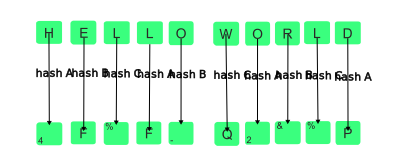
\includegraphics[width=0.7\linewidth]{img/helloworld.png}
  \caption{Encrypting \textit{hello world} with a periodically-repeating stream of 3 shuffled keyboards.}
  \label{fig:helloworld}
\end{figure}


The seeds used to generate the new keyboard, rather than the specific keyboard arrangement, are the objects kept in memory throughout the encryption. 
As suggested above, the decryption takes the keys used to encrypt the messages and reverses the protocol. 
This method, thus, optimizes auxiliary space, $\mathcal{O}(N)$, rather than encryption time complexity, $\mathcal{O}(MC)$, 
where $N$ is the number of digits of the $\mathrm{key_2}$, while $M$ and $K$ are the message 
length and number of keyboard characters to encrypt, respectively.




\end{document}